\documentclass{standalone}
\usepackage{tikz}
\usetikzlibrary{quantikz}

\begin{document}

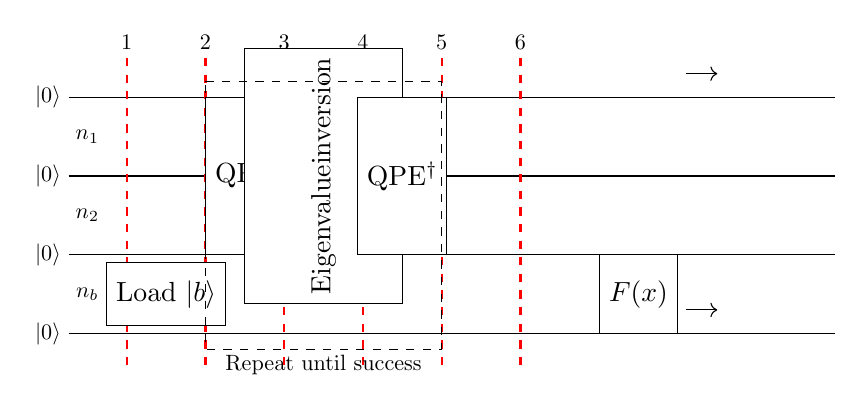
\begin{tikzpicture}

% Define qubit wires
\node[scale=0.8] (q0) at (0,2) {$\vert 0 \rangle$};
\node[scale=0.8] (q1) at (0,1) {$\vert 0 \rangle$};
\node[scale=0.8] (q2) at (0,0) {$\vert 0 \rangle$};
\node[scale=0.8] (q3) at (0,-1) {$\vert 0 \rangle$};

% Draw qubit wires
\draw (q0) -- (10,2);
\draw (q1) -- (10,1);
\draw (q2) -- (10,0);
\draw (q3) -- (10,-1);

% Add measure symbols
\node[scale=0.8] (m1) at (8,2.3) {};
\node[scale=0.8] (m2) at (8,-0.7) {};
\draw[->] (m1) -- ++(0.5,0);
\draw[->] (m2) -- ++(0.5,0);

% Add labels to qubit wires
\node[scale=0.8] at (0.5,1.5) {$n_1$};
\node[scale=0.8] at (0.5,0.5) {$n_2$};
\node[scale=0.8] at (0.5,-0.5) {$n_b$};

% Add vertical dashed lines
\foreach \x in {1,2,3,4,5,6} {
  \draw[dashed,red,thick] (\x,2.5) -- (\x,-1.5);
  \node[scale=0.8] at (\x,2.7) {\x};
}

% Add boxes
\node[draw,minimum width=1cm,minimum height=0.8cm,fill=white] (load) at (1.5,-0.5) {Load $\vert b \rangle$};
\node[draw,minimum width=1cm,minimum height=2cm,fill=white] (qpe1) at (2.5,1) {QPE};
\node[draw,minimum width=1cm,minimum height=2cm,fill=white,rotate=90] (eiginv) at (3.5,1) {Eigenvalue\\inversion};
\node[draw,minimum width=1cm,minimum height=2cm,fill=white] (qpe2) at (4.5,1) {QPE$^\dagger$};
\node[draw,minimum width=1cm,minimum height=1cm,fill=white] (fx) at (7.5,-0.5) {$F(x)$};

% Add dashed box around QPE and eigenvalue inversion
\draw[dashed] (2,2.2) -- (5,2.2) -- (5,-1.2) -- (2,-1.2) -- cycle;
\node[scale=0.8] at (3.5,-1.4) {Repeat until success};

\end{tikzpicture}

\end{document}